%% LyX 2.3.6 created this file.  For more info, see http://www.lyx.org/.
%% Do not edit unless you really know what you are doing.
\documentclass[a4paper,english]{scrartcl}
\usepackage[T1]{fontenc}
\usepackage[latin9]{inputenc}
\usepackage{graphicx}

\makeatletter

%%%%%%%%%%%%%%%%%%%%%%%%%%%%%% LyX specific LaTeX commands.
\pdfpageheight\paperheight
\pdfpagewidth\paperwidth


\makeatother

\usepackage{babel}
\usepackage{listings}
\renewcommand{\lstlistingname}{Listing}

\begin{document}
\title{SEA3004F M2P1-memo: Properties of the atmosphere}
\author{Ocean and Atmosphere Dynamics}
\maketitle

\section{Approximated saturation vapour pressure {[}20 marks{]}}

This part was merely the execution of the commands given in the tutorial.
The final figure is shown in Fig. \ref{fig:Result1} (there should
also be a title). If there is neither a figure nor code, the mark is 0. Please
check the code and give 5-7 points depending on how close to the tutorial
it was. Mark down -8 if the units are wrong (i.e. they used degree
C as input) and -2.5 for every wrong or missing annotation (axes and
title);

\begin{figure}
\centering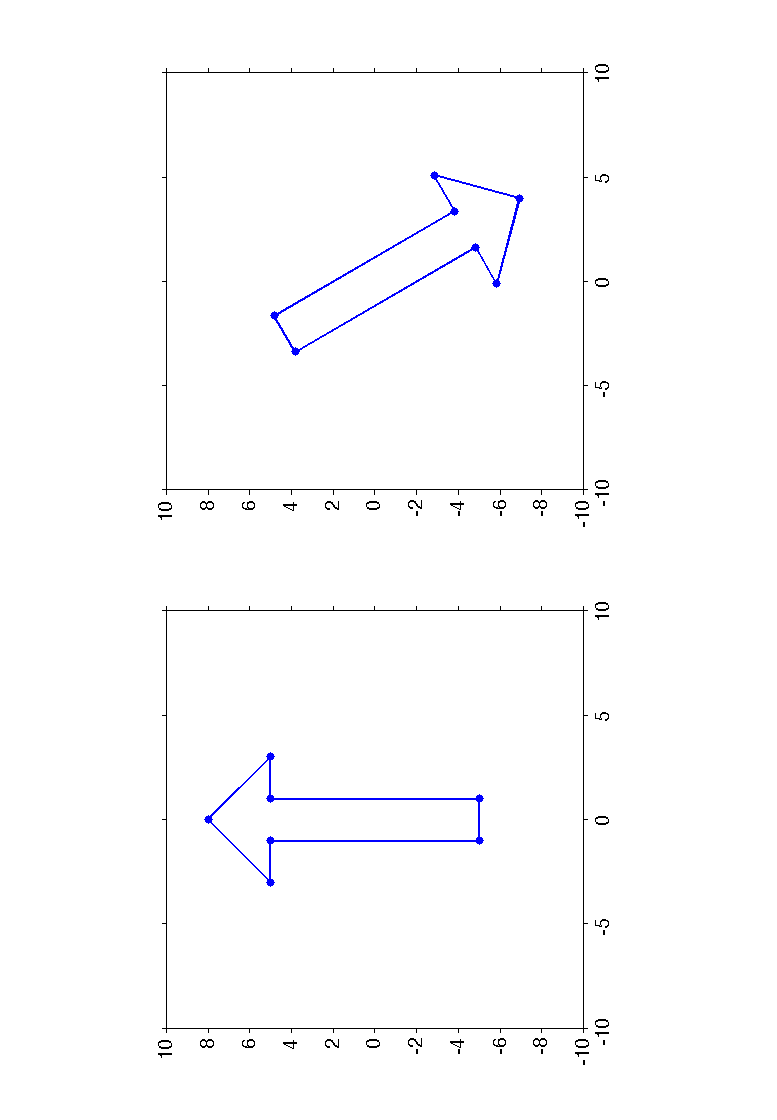
\includegraphics[scale=0.6]{fig1}

\caption{\label{fig:Result1}Exercise 1}

\end{figure}


\section{Water vapour in the standard atmosphere {[}50 marks{]}}
\begin{enumerate}
\item Using your function to compute the saturation vapour pressure as a
function of temperature T and the equation of state of water vapour,
compute the maximum amount of water vapour per unit volume that air
can hold at the surface and at a height of 10 km. The temperature
values for the 2 heights can be obtained with the standard atmosphere
function presented in the tutorial. \\
\textbf{{[}20 marks{]}} The students are expected to show how they
obtained the results in the code. Mark down -7 if the result is correct
but given without any comment in the code; mark down -5 if the value
of the gas constant is the one for the ideal gases (it should be for
water vapour); mark down -5 if the values are wrong because of wrong
pressure or wrong temperature, (-5 for each). Answer: 
\begin{lstlisting}[language=Matlab,basicstyle={\small\ttfamily},showstringspaces=false,frame=lines]
z=[0 10000]; 
temp=tstdatm(z)    % obtain temperature for the standard atmosphere [K] 
temp = 288.1500  223.1500
svpa(temp)=  1669.20    21.327 % saturation vapour pressure [Pa]
\end{lstlisting}
then apply the \emph{equation of state for water vapour 
\[
p_{v}=\rho_{v}R_{v}T_{v}
\]
using 
\[
R_{v}=\frac{R_{g}}{m_{v}}=\frac{8.3143}{18.016\,10^{-3}}=461\ J\,kg^{-1}\,K^{-1}
\]
to get
\[
\rho_{v}(surf)=\frac{p_{v}}{R_{v}T_{v}}=\frac{1669.2}{461\times288.15}=12.6\times10^{-3}\,kg\,m^{-3}
\]
\[
\rho_{v}(10km)=\frac{p_{v}}{R_{v}T_{v}}=\frac{21.327}{461\times233.15}=1.98\times10^{-4}\,kg\,m^{-3}
\]
In case someone uses a function to compute density, standing ovation
and add a bonus of 5 marks (I would be VERY surprised...)} 
\item Write a MATLAB script to plot the saturation vapour pressure as a
function of the standard atmosphere temperature from the surface to
the height of 20 km in steps of 500 m. The results of both functions
(\texttt{svp} and \texttt{svpa}) must be shown and the legend must
identify the lines. Put the units of the Y-axis in km and the units
of the X-axis in hPa. The resulting figure is shown in Fig.\textbf{
}\\
\textbf{{[}30 marks{]}} Mark down -5 if the units are wrong; -7 if
there are no units or no labels at all; -5 if there is no legend (no
matter what the text in the legend is, as long as it is clear). -5
if the script is not commented 
\begin{lstlisting}[language=Matlab,basicstyle={\small\ttfamily},showstringspaces=false,frame=lines]
z=0:500:20000;      % define height at discrete steps [m]
temp=tstdatm(z);    % obtain temperature for the standard atmosphere [K]
svpa20=svpa(temp);  % compute appx svp [Pa]
svp20=svp(temp);    % compute svp [Pa]

figure
plot(svpa20/100,z/1000,'b')     % plot svpa in hPa and km
hold on
plot(svp20/100,z/1000,'r')      % plot svp in hPa and km
legend('Approximated','Goff & Gratch (1946)')
xlabel('Saturation Vapour Pressure [hPa]')
ylabel('Height [km]')
\end{lstlisting}
\end{enumerate}
\begin{figure}
\centering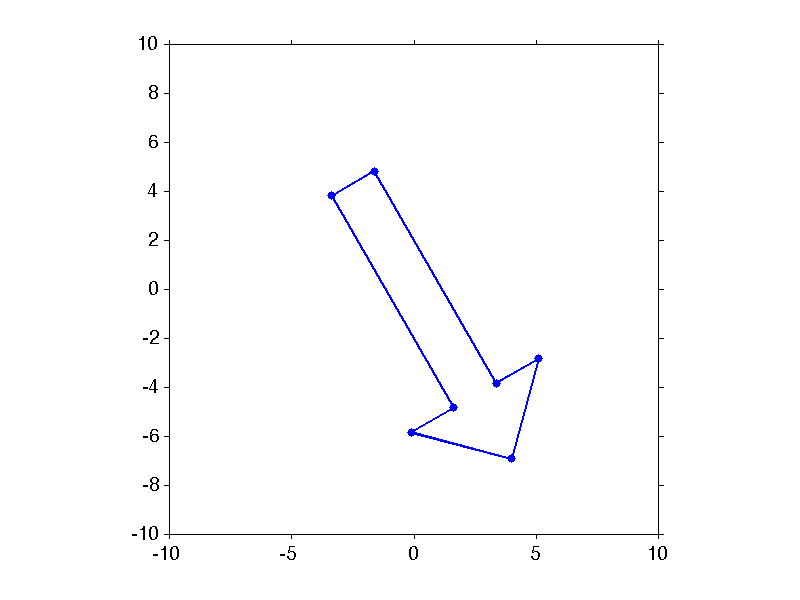
\includegraphics[scale=0.5]{fig2}

\caption{Exercise 3}

\end{figure}

\end{document}
